\section{Marco teórico}

\subsection{La familia SQuaRE}

SQuaRE agrupa normas para especificar, modelar, medir y evaluar la calidad de sistemas y software. ISO/IEC 25010 define modelos de calidad; ISO/IEC 25022 se concentra en medidas de calidad en uso; e ISO/IEC 25040 orienta el proceso de evaluación \cite{iso25010,iso25022,iso25040}. Estas normas cumplen funciones relacionadas, pero no intercambiables.

\begin{figure}[H]
\centering
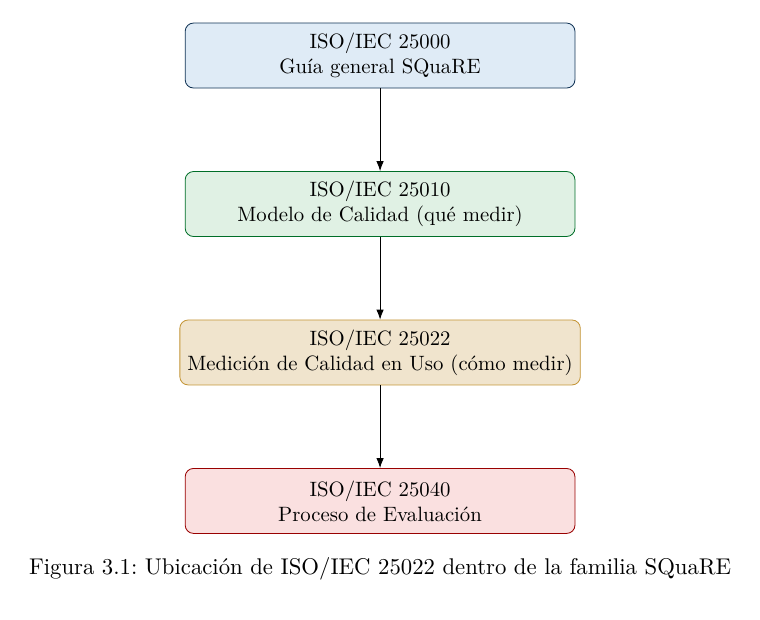
\includegraphics[width=.88\textwidth]{figures/square.png}
\caption{Ubicación de ISO/IEC 25022 en la familia SQuaRE.}
\label{fig:square}
\end{figure}

\scenario{3}{Comprensión del modelo SQuaRE · fuente literal}

La Figura \ref{fig:square} permite distinguir tres preguntas: \emph{qué propiedades se esperan}, \emph{cómo se medirán} y \emph{cómo se ejecutará la evaluación}. En este trabajo, el modelo de calidad sirve para establecer las dimensiones relevantes; las medidas convierten los eventos en valores comparables; y el proceso de evaluación conserva la relación entre requisito, evidencia, cálculo y decisión.

\subsection{Calidad interna, externa y en uso}

Los tres niveles observan el sistema desde perspectivas diferentes. La calidad interna analiza artefactos sin ejecutar el producto; la externa estudia su comportamiento durante pruebas; y la calidad en uso examina los resultados obtenidos por personas al realizar tareas dentro de un contexto.

\begin{table}[H]
\centering
\caption{Niveles de calidad aplicados a MediSalud HIS}
\begin{tabularx}{\textwidth}{p{2.6cm}YY}
\toprule
\textbf{Nivel} & \textbf{Objeto de observación} & \textbf{Aplicación al caso} \\
\midrule
Interna & Código, arquitectura, dependencias y estructura estática & Complejidad, duplicación, cobertura de pruebas y separación de responsabilidades del servicio HCE. \\
Externa & Comportamiento del producto ejecutado en un entorno de prueba & Respuesta del Gateway, persistencia de una nota o entrega de un evento RabbitMQ bajo una prueba controlada. \\
En uso & Resultado, esfuerzo, percepción y riesgo para un usuario en una tarea y contexto & Tiempo que requiere un médico para guardar una nota, abandono del paciente al agendar o daño potencial de una receta incorrecta. \\
\bottomrule
\end{tabularx}
\end{table}

Un sistema puede tener código mantenible y aun así ofrecer una experiencia deficiente. Del mismo modo, una API puede superar pruebas funcionales y fallar para una sede con conectividad limitada. Por ello, herramientas de análisis estático no sustituyen la observación de tareas ni las métricas de calidad en uso.

\subsection{Características de calidad en uso}

\subsubsection{Efectividad}

Expresa la exactitud e integridad con la que los usuarios alcanzan sus objetivos. En MediSalud se materializa en la proporción de citas completadas, recetas correctas, registros sincronizados o resultados visualizados. Una tarea puede terminar técnicamente y no ser efectiva si conserva datos incompletos o equivocados.

\subsubsection{Eficiencia}

Relaciona los resultados alcanzados con los recursos consumidos. El recurso más visible es el tiempo, aunque también pueden medirse pasos, interacciones o esfuerzo. En el caso se emplean percentiles porque el promedio oculta a los usuarios que experimentan las respuestas más lentas.

\subsubsection{Satisfacción}

Representa el grado en que las necesidades del usuario quedan satisfechas. Incluye utilidad percibida, confianza, agrado y comodidad. Se observa mediante CSAT y abandono de encuestas; estas medidas se interpretan junto con las tareas y no como una valoración aislada de interfaz.

\subsubsection{Libertad de riesgo}

Considera la mitigación de consecuencias negativas económicas, de salud, seguridad y ambiente. En un HIS tiene prioridad especial: una alergia ausente o una dosis incorrecta puede afectar al paciente; una factura duplicada produce daño financiero; y una exposición de datos compromete privacidad y confianza.

\subsubsection{Cobertura del contexto}

Determina si el sistema mantiene calidad en los contextos previstos y si puede adaptarse más allá de ellos. MediSalud opera en varias sedes y combina escritorio, móvil, red hospitalaria y conexiones domésticas. La variabilidad entre sedes y las caídas de teleconsulta permiten observar esta característica.

\subsection{Modelo usuario--tarea--contexto}

La unidad de análisis no es el módulo por sí solo, sino la combinación usuario--tarea--contexto (UTC). Por ejemplo, ``guardar HCE'' cambia de significado cuando se realiza durante una consulta en hora pico, desde una sede remota o con información de alergias no disponible. El modelo evita asignar una característica ISO únicamente por palabras clave y obliga a justificar el efecto real del incidente.

\begin{table}[H]
\centering
\caption{Ejemplos de unidades UTC}
\begin{tabularx}{\textwidth}{p{2.2cm}p{3.5cm}Yp{3cm}}
\toprule
Usuario & Tarea & Contexto & Característica principal \\
\midrule
Médico & Guardar nota de evolución & Consulta externa, hora pico, sede Quito & Eficiencia \\
Paciente & Agendar una cita & Teléfono móvil y conexión 4G & Efectividad / satisfacción \\
Farmacia & Validar una prescripción & Turno nocturno de urgencias & Libertad de riesgo \\
Paciente & Completar teleconsulta & Domicilio y WiFi limitado & Cobertura del contexto \\
Admisión & Emitir factura con seguro & Cierre mensual & Libertad de riesgo \\
\bottomrule
\end{tabularx}
\end{table}
